% ======================================================================
% Modelo de Decisión para Aprobación de Créditos y Segmentación de Riesgo
% Presentación — Administración Actuarial (Licenciatura en Actuaría)
% Compilar: pdflatex presentacion.tex (x2)
% ======================================================================
\documentclass[10pt,aspectratio=169]{beamer}

\usepackage[T1]{fontenc}
\usepackage[utf8]{inputenc}
\usepackage[spanish,mexico]{babel}
\usepackage{booktabs}
\usepackage{graphicx}
\usepackage{amsmath}
\usepackage{xcolor}

\definecolor{azul}{RGB}{11,83,148}
\definecolor{azulfuerte}{RGB}{8,55,99}
\usetheme{Madrid}
\usecolortheme{whale}
\setbeamercolor{structure}{fg=azulfuerte}
\setbeamercolor{title}{fg=white,bg=azulfuerte}
\setbeamercolor{frametitle}{fg=azulfuerte}
\setbeamercolor{block title}{bg=azul,fg=white}
\setbeamercolor{block body}{bg=azul!8,fg=black}
\setbeamertemplate{navigation symbols}{}
\setbeamertemplate{caption}{\insertcaption}

\title[Modelo de Decisión de Crédito]{Modelo de Decisión para la Aprobación
  de Créditos y Segmentación de Riesgo}
\subtitle{Administración Actuarial --- Licenciatura en Actuaría}
\author{Orlando Barcena Romero}
\institute{Facultad de Estudios Superiores Acatlán, UNAM}
\date{Ciclo escolar 2025--2026}

\begin{document}

% ----------------------------------------------------------------------
\begin{frame}<beamer>
  \titlepage
\end{frame}

% ----------------------------------------------------------------------
\begin{frame}{Agenda}
  \tableofcontents
\end{frame}

% ----------------------------------------------------------------------
\section{Planteamiento del problema}
\begin{frame}{Planteamiento del problema}
  \begin{block}{Restricción operativa}
    La institución \textbf{aprueba solo el 25\%} de las solicitudes de crédito
    recibidas y requiere clasificar a los aceptados en segmentos de riesgo.
  \end{block}
  \begin{itemize}
    \item \textbf{Selección:} elegir el 25\% de solicitantes con menor riesgo.
    \item \textbf{Segmentación:} dentro de los aprobados, separar \emph{Buenos}
          (bajo riesgo) y \emph{Malos} (riesgo controlado).
  \end{itemize}
  \vspace{0.5em}
  \begin{alertblock}{Pregunta}
    \begin{center}
      ¿Puede un modelo estadístico validado superar al criterio de reglas de
      la práctica tradicional, a igual tasa de aprobación?
    \end{center}
  \end{alertblock}
\end{frame}

% ----------------------------------------------------------------------
\section{Datos}
\begin{frame}{Datos: Lending Club}
  \begin{columns}
    \begin{column}{0.58\linewidth}
      \begin{itemize}
        \item \textbf{292{,}849} solicitudes de crédito personal,
              2007--2015.
        \item 42 variables disponibles: solicitud y desempeño del préstamo.
        \item \emph{Mal préstamo} = recuperación de principal $< 70\%$
              (proxy de incumplimiento).
      \end{itemize}
      \vspace{0.4em}
      Resultado global: \textbf{72.1\%} de malos.
      \vspace{0.8em}
      \begin{block}{Sin leakage}
        El modelo solo usa variables \textbf{disponibles en la solicitud}.
      \end{block}
    \end{column}
    \begin{column}{0.42\linewidth}
      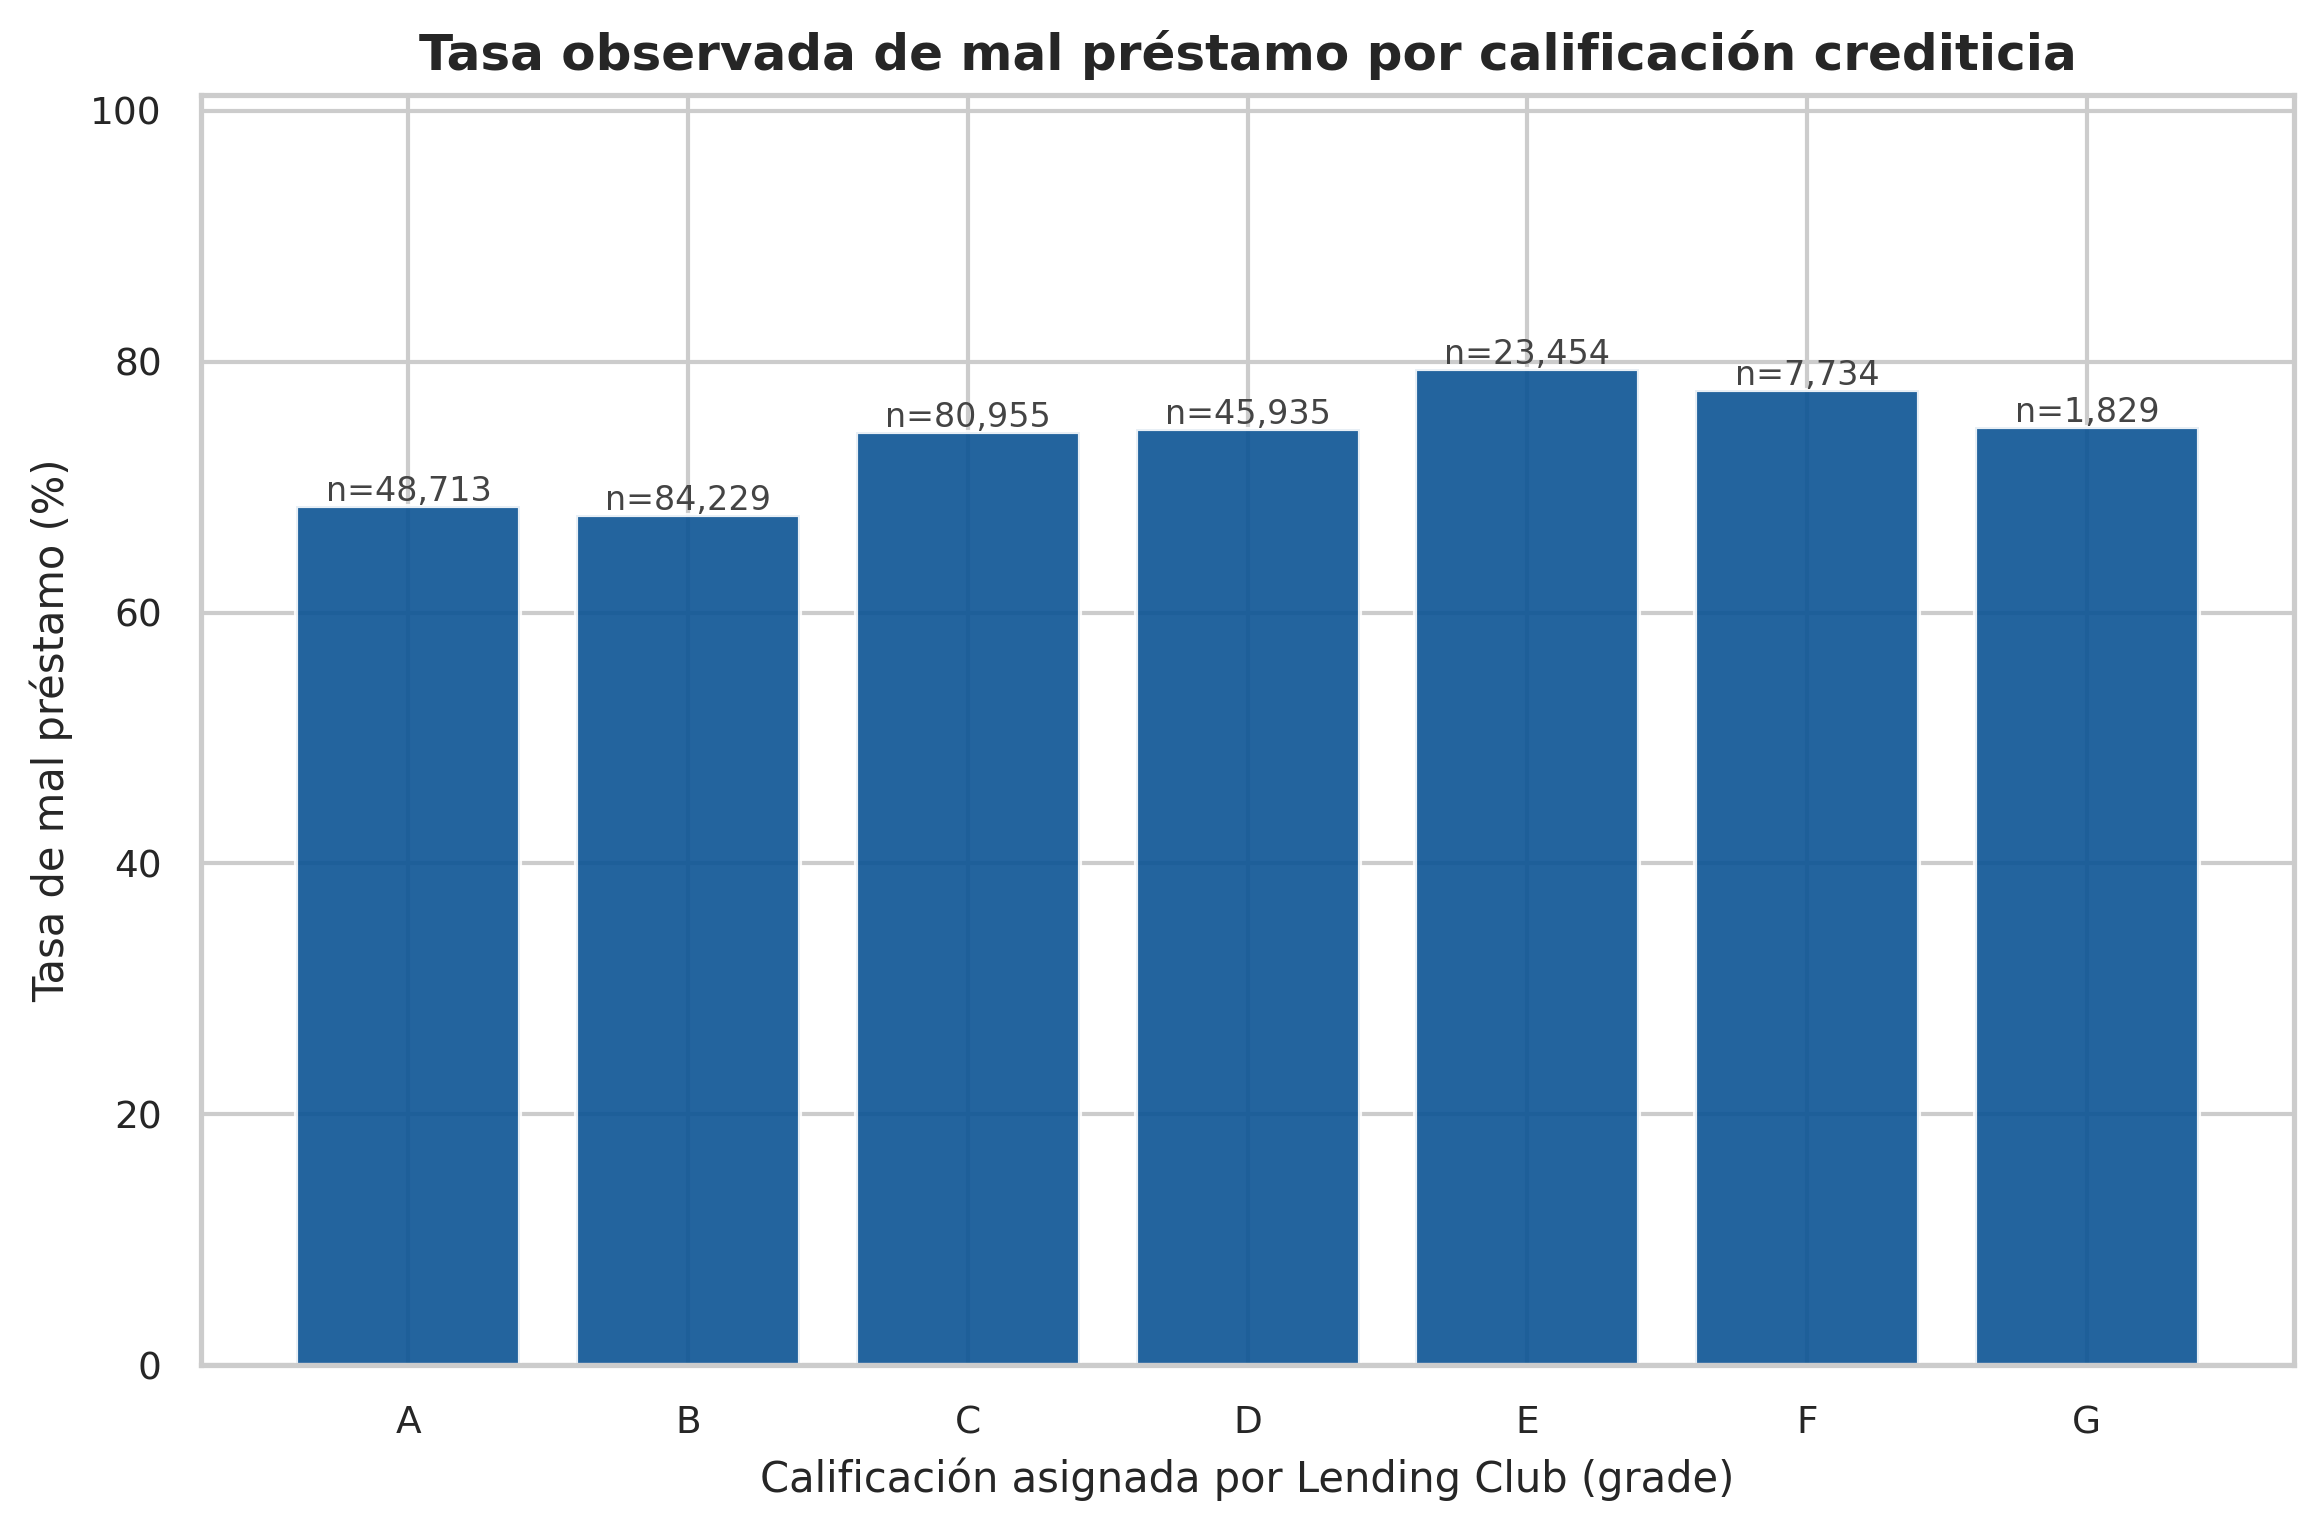
\includegraphics[width=\linewidth]{figuras/eda_bad_rate_by_grade.png}
    \end{column}
  \end{columns}
\end{frame}

% ----------------------------------------------------------------------
\section{Metodología}
\begin{frame}{Metodología}
  \begin{enumerate}
    \item \textbf{Objetivo:} préstamo malo si recuperación $< 70\%$.
    \item \textbf{Modelo:} regresión logística sobre 44 variables de
          solicitud, train/test 70/30 estratificado.
    \item \textbf{Scorecard:} escala de puntos tipo FICO
          \begin{equation*}
            \text{Score} = \text{offset} - 28.85\,\ln\!\left(\frac{p}{1-p}\right)
            \qquad \text{(20 pts por duplicar el odds)}
          \end{equation*}
    \item \textbf{Umbrales} (calibrados solo en entrenamiento):
          \begin{itemize}
            \item Score $\geq 600$ (cuantil 25\% de riesgo) $\rightarrow$ \textbf{Aprobado}.
            \item Score $\geq 613$ dentro de aprobados $\rightarrow$ \textbf{Bueno}; si no, \textbf{Malo}.
          \end{itemize}
  \end{enumerate}
\end{frame}

\begin{frame}{Validación: muestras independientes}
  \begin{table}
    \small
    \begin{tabular}{lccc}
      \toprule
      Muestra & AUROC & GINI & KS \\
      \midrule
      Entrenamiento ($n = 204{,}994$) & 0.7462 & 0.4924 & 0.3702 \\
      Test ($n = 87{,}855$)           & 0.7462 & 0.4924 & 0.3700 \\
      \bottomrule
    \end{tabular}
  \end{table}
  \vspace{0.6em}
  \begin{itemize}
    \item Idénticas en train y test $\rightarrow$ \textbf{sin sobreajuste}.
    \item AUROC 0.75: separación buena, comparable a banca minorista.
  \end{itemize}
  \vspace{0.5em}
  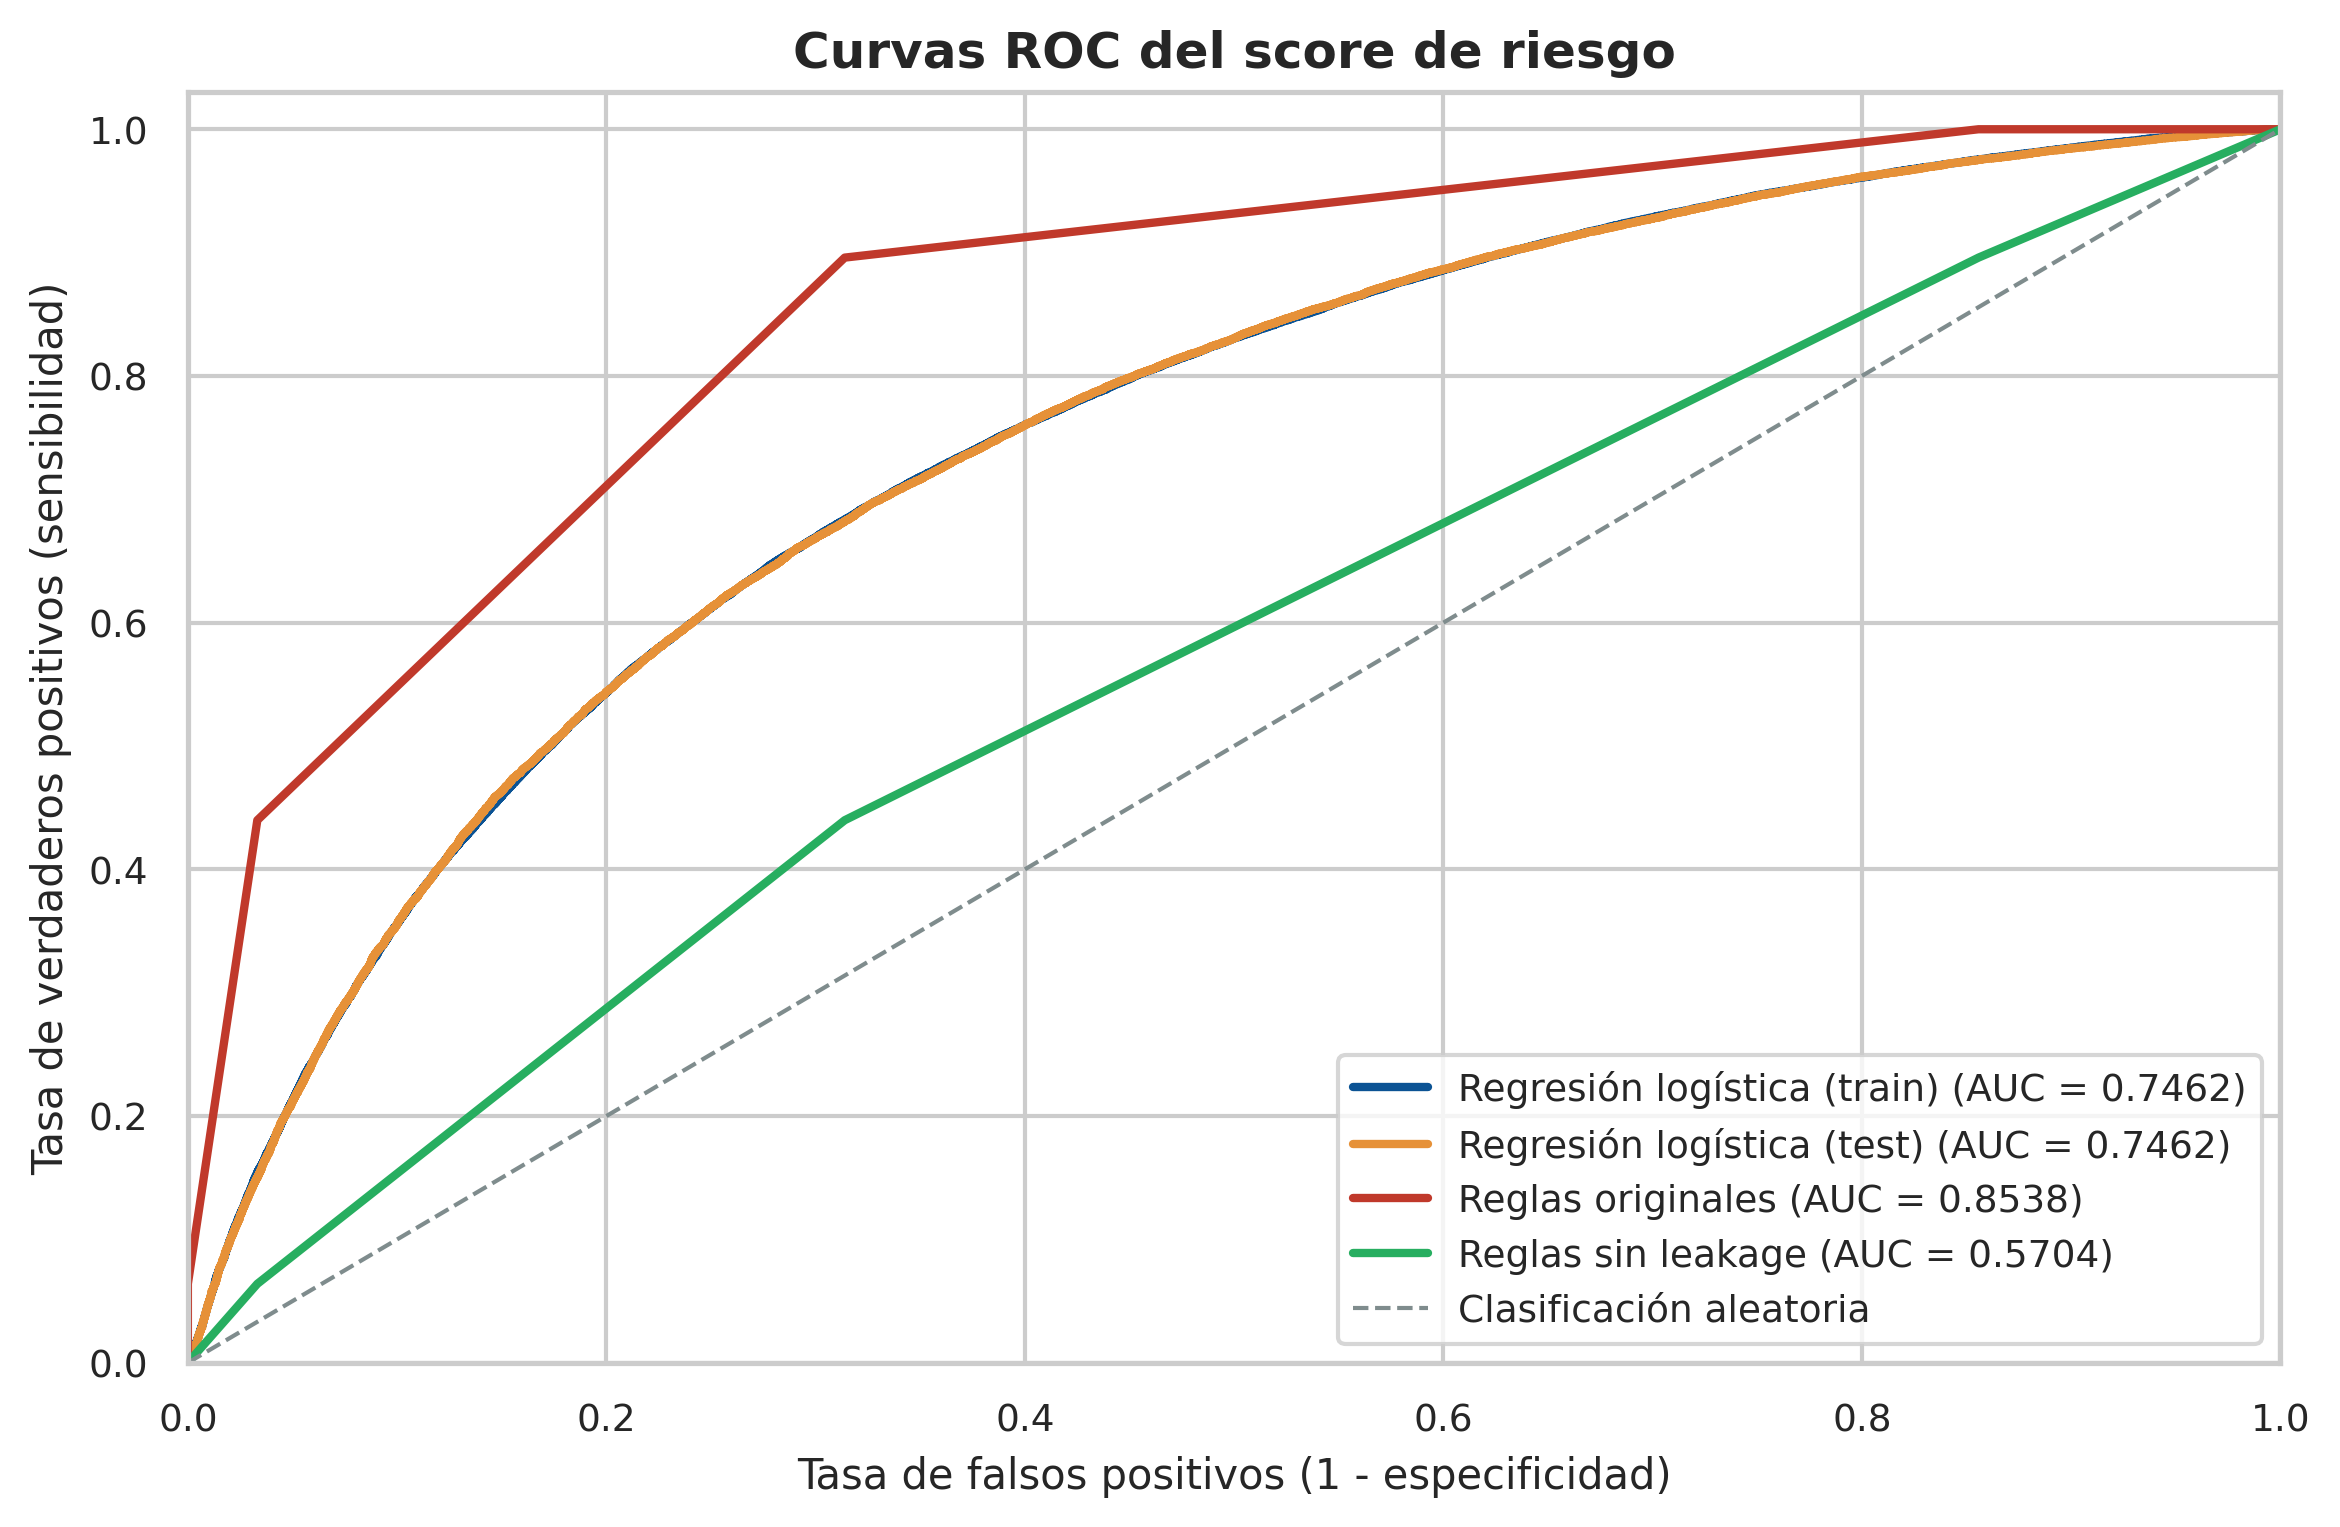
\includegraphics[width=0.78\linewidth]{figuras/model_roc.png}
\end{frame}

% ----------------------------------------------------------------------
\section{Resultados}
\begin{frame}{Resultados I: política de aprobación (test)}
  \begin{columns}
    \begin{column}{0.5\linewidth}
      \begin{table}
        \small
        \begin{tabular}{lc}
          \toprule
          Indicador & Valor \\
          \midrule
          Tasa de aprobación & \textbf{24.9\%} \\
          Malos en aprobados & 45.8\% \\
          Malos en rechazados & 80.8\% \\
          Malos globales & 72.1\% \\
          Captura de malos & \textbf{84.2\%} \\
          \bottomrule
        \end{tabular}
      \end{table}
      \begin{itemize}
        \item La cartera aprobada casi \textbf{duplica} la calidad de la
              población.
        \item 84 de cada 100 incumplidos quedan fuera de la cartera con solo
              revisar el 25\% de menor riesgo.
      \end{itemize}
    \end{column}
    \begin{column}{0.5\linewidth}
      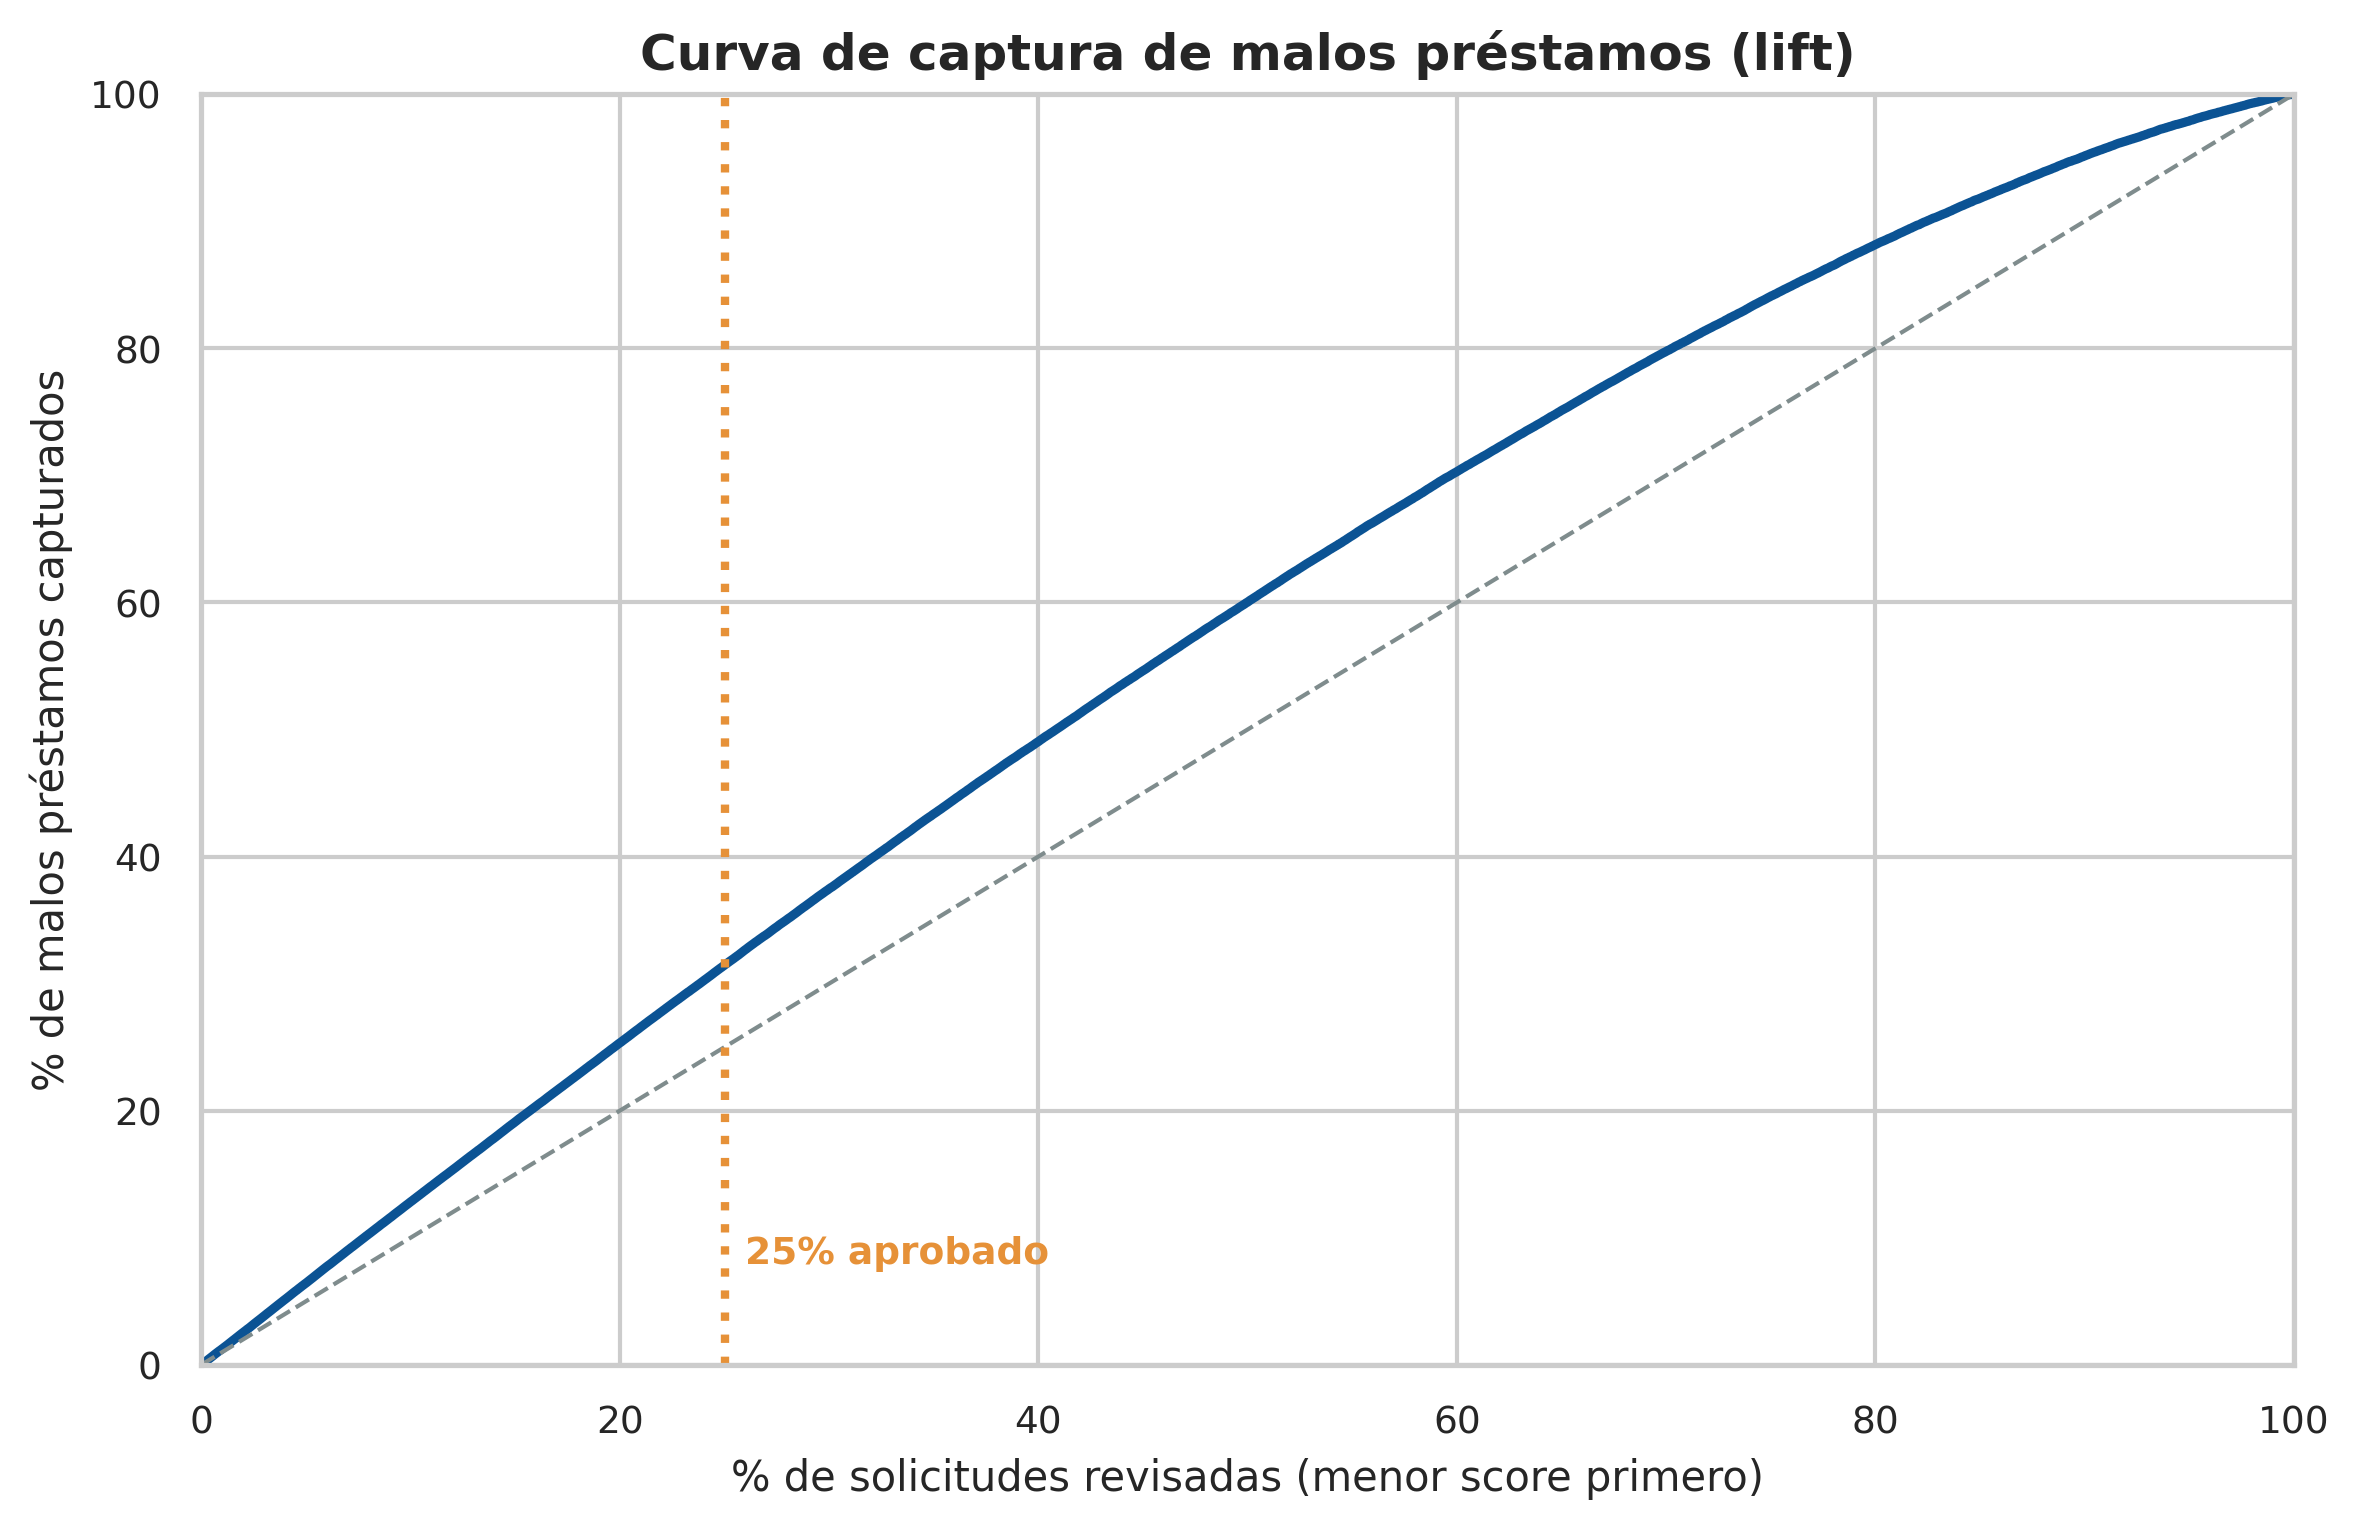
\includegraphics[width=\linewidth]{figuras/model_lift_chart.png}
    \end{column}
  \end{columns}
\end{frame}

\begin{frame}{Resultados II: segmentación de aprobados}
  \begin{columns}
    \begin{column}{0.52\linewidth}
      \begin{block}{Segmento Bueno --- $n = 11{,}091$}
        Malos: \textbf{37.5\%}\\ Tratamiento preferente: tasa y límites
        estándar.
      \end{block}
      \begin{block}{Segmento Malo --- $n = 10{,}766$}
        Malos: \textbf{54.3\%}\\ Monitoreo intensivo y provisiones mayores.
      \end{block}
      \begin{itemize}
        \item La mediana del score dentro de aprobados separa carteras con
              \textbf{17 puntos} de diferencia en morosidad.
      \end{itemize}
    \end{column}
    \begin{column}{0.48\linewidth}
      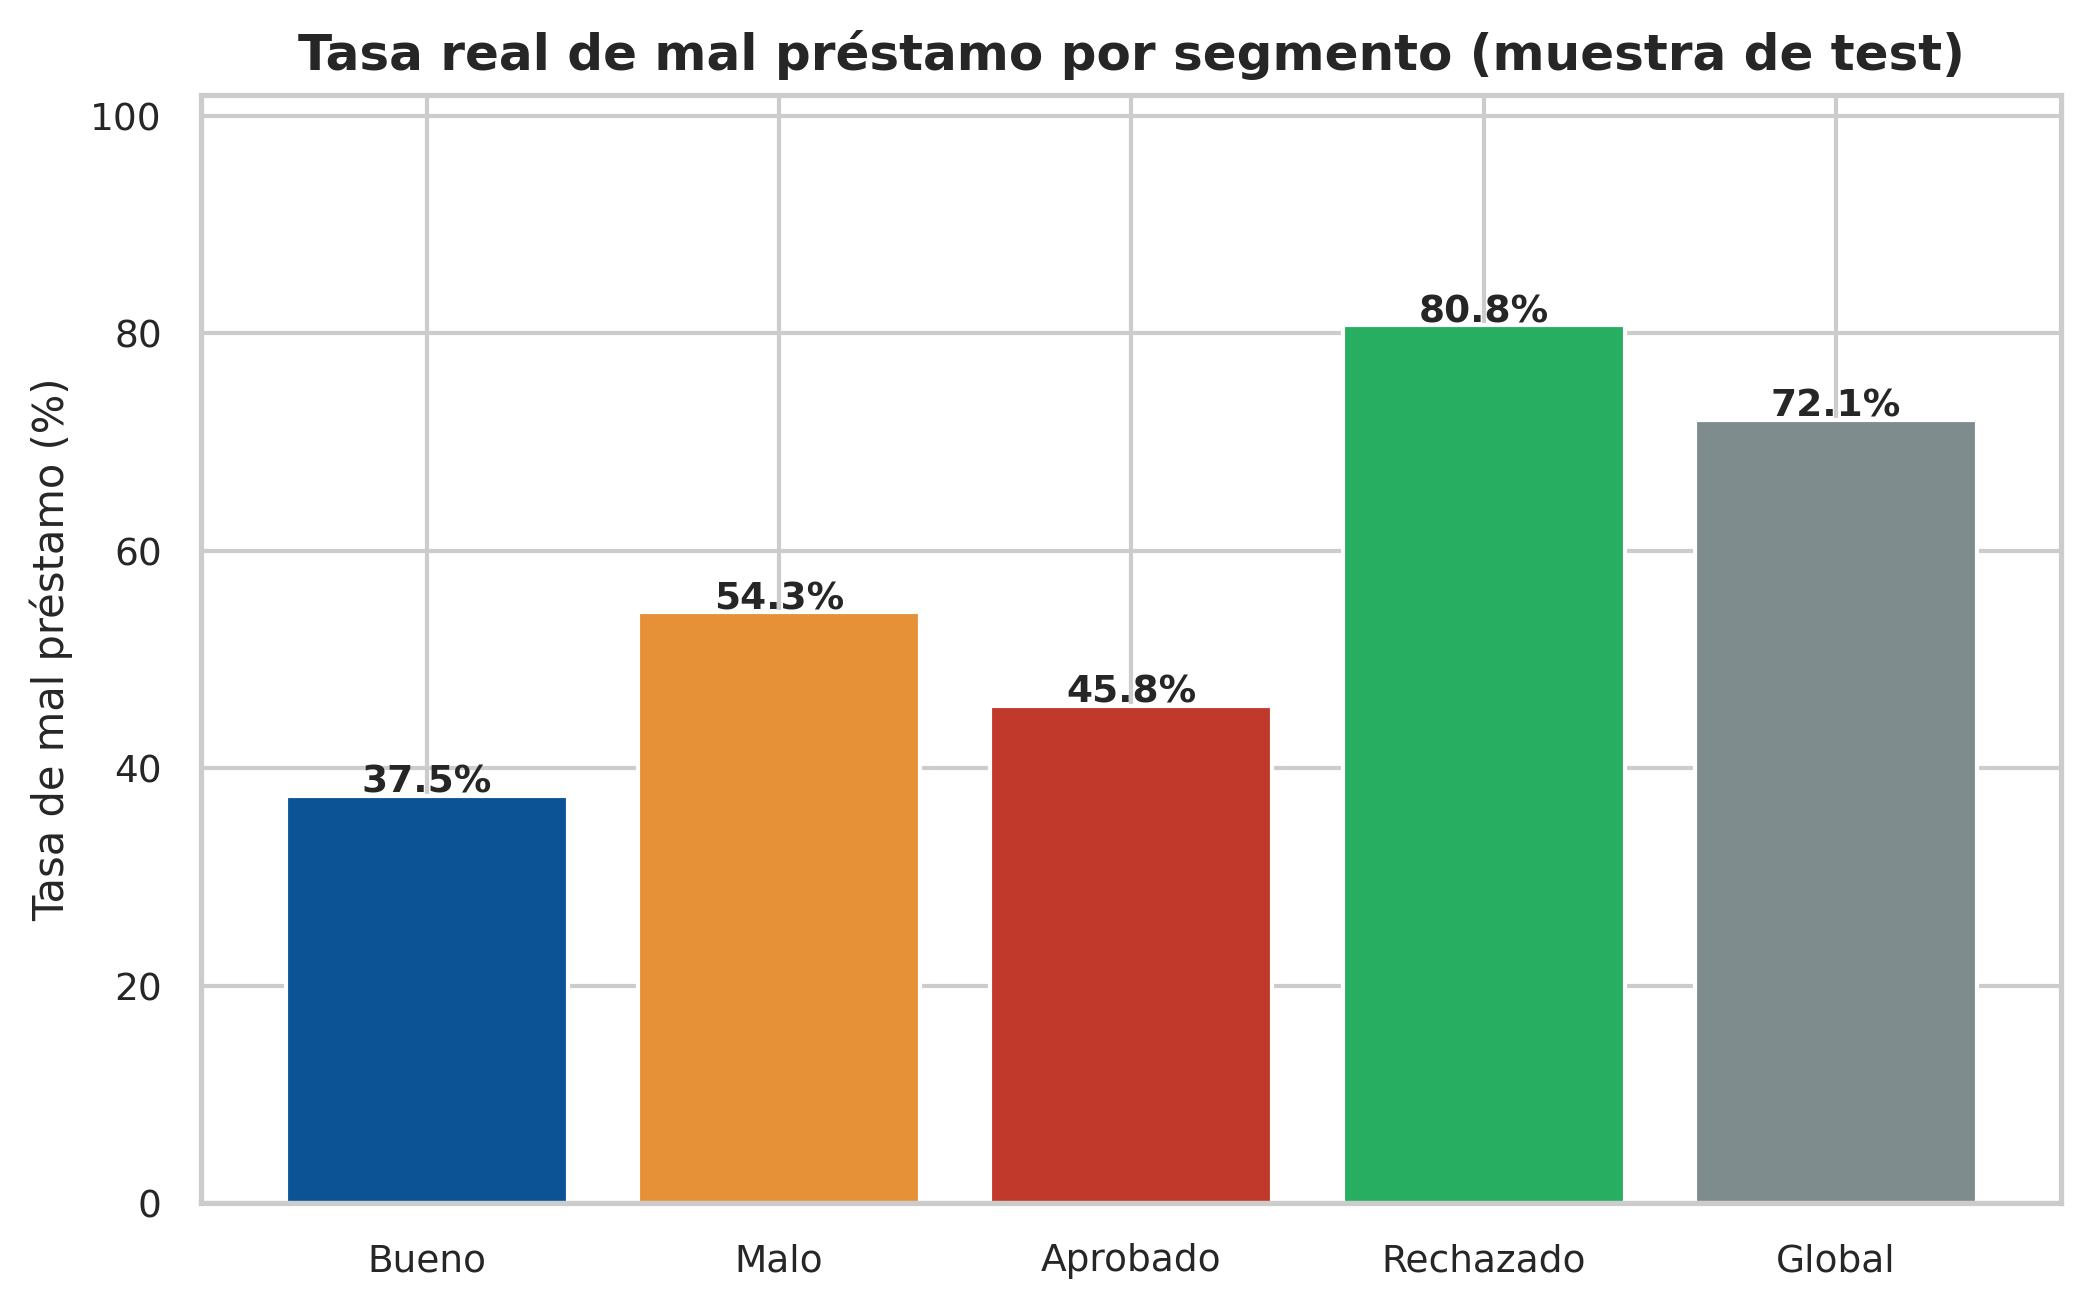
\includegraphics[width=\linewidth]{figuras/model_approval_rates.png}
    \end{column}
  \end{columns}
\end{frame}

% ----------------------------------------------------------------------
\section{Comparación con el modelo de reglas}
\begin{frame}{Comparación: estadístico vs.\ modelo de reglas (25\%)}
  \begin{table}
    \small
    \begin{tabular}{lcc}
      \toprule
      Método & AUROC & Malos en cartera aprobada \\
      \midrule
      \textbf{Regresión logística (test)} & \textbf{0.746} & \textbf{45.8\%} \\
      Reglas del ejercicio, sin recuperación & 0.570 & 67.8\% \\
      Reglas del ejercicio, con recuperación & 0.854 & 28.6\% \\
      \bottomrule
    \end{tabular}
  \end{table}
  \vspace{0.6em}
  \begin{alertblock}{Lección metodológica}
    La variante \emph{con recuperación} usa la variable de resultado dentro de
    la regla de decisión (\textbf{leakage}): sus métricas lucen superiores pero
    no son alcanzables en la práctica. El modelo estadístico opera con
    información real de solicitud y reduce \textbf{un tercio} la morosidad de
    la cartera (67.8\% $\rightarrow$ 45.8\%).
  \end{alertblock}
\end{frame}

% ----------------------------------------------------------------------
\section{Conclusiones}
\begin{frame}{Conclusiones}
  \begin{enumerate}
    \item Scorecard logístico validado: \textbf{AUROC 0.746}, sin sobreajuste.
    \item Tasa de aprobación efectiva \textbf{24.9\%} (objetivo 25\%).
    \item Cartera aprobada con 45.8\% de malos vs.\ 72.1\% poblacional;
          \textbf{84\%} de incumplidos excluidos.
    \item Sub-segmentación operativa: Bueno 37.5\% vs.\ Malo 54.3\%.
    \item Detecta y corrige el leakage del ejercicio original; mejora un
          tercio la calidad de cartera frente a las reglas operables.
  \end{enumerate}
  \vspace{0.8em}
  \begin{block}{Trabajo futuro}
    Objetivo regulatorio (\emph{charge-off}), validación temporal por
    cohortes, modelos alternativos (Gradient Boosting), capital económico y
    rentabilidad ajustada por riesgo.
  \end{block}
\end{frame}

% ----------------------------------------------------------------------
\begin{frame}{Gracias}
  \centering
  \vspace{1.2em}
  {\Large\textbf{Modelo de Decisión para la Aprobación de Créditos}}\\[0.4em]
  {\large y Segmentación de Riesgo}\\[1.5em]
  Administración Actuarial --- Licenciatura en Actuaría\\[0.4em]
  \textbf{Orlando Barcena Romero}\\[0.4em]
  Facultad de Estudios Superiores Acatlán, UNAM\\[1.2em]
  \small
  Informe y código reproducibles en el repositorio del proyecto.\\[0.3em]
  Datos: Lending Club (públicos) --- \texttt{run\_pipeline.py} reproduce todo el análisis.
\end{frame}

\end{document}